\documentclass{standalone}
\usepackage{tikz}
\usetikzlibrary{positioning}

\tikzset{
	sinesym/.pic = {
	 \draw [domain=0:2, samples=200] plot (\x, {sin(180*\x)/3});}}
\tikzset{
	osc/.pic = {
	 \coordinate (-inleft) at (-0.8,0) ;
	 \coordinate (-inright) at (0.8,0) ;
	 \coordinate (-out) at (0,-1.5) ;
	 \coordinate (-center) at (0,-0.7) ;
	 \coordinate (-right) at (1.3,-.7) ;
	 \coordinate (-left) at (-1.3,-.7) ;
	 \draw (-1.5,0) -- (1.5,0) arc (0:-180:1.5) --cycle;
	 \pic [scale=1/3] at (-.35,-.7) {sinesym};
	 }
	}
	

\begin{document} \sffamily
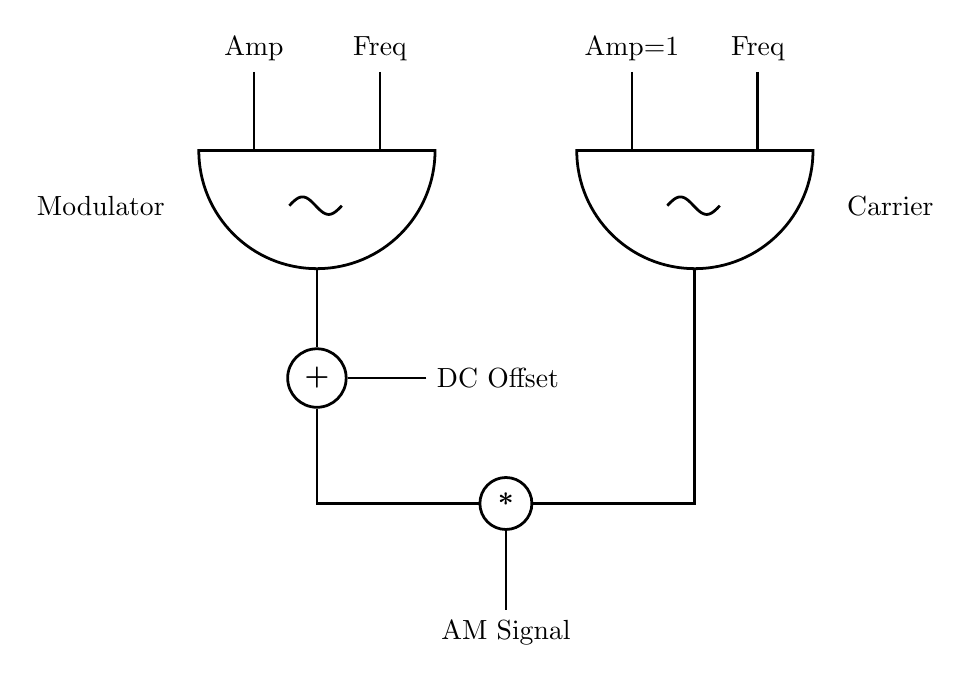
\begin{tikzpicture}[node distance=1, line width=1pt]

% NODES
% modulator
\pic (mod) {osc};
\node (modlabel) [left=of mod-left, xshift=0.5cm] {Modulator};
\node (mamp) [above=of mod-inleft] {Amp};
\node (mfreq) [above=of mod-inright] {Freq};
% carrier
\pic (car) [right=of mod-inright, xshift=3cm] {osc};
\node (camp) [above=of car-inleft] {Amp=1};
\node (cfreq) [above=of car-inright] {Freq};
\node (carlabel) [right=of car-right, xshift=-0.5cm] {Carrier};
% plus, mult, out
\node (plus) [circle, draw=black, below=of mod-out, font=\bfseries] {+};
\node (dc) [right=of plus] {DC Offset};
\path (car-out) -- (mod-out) node (middle) [midway]{};
\node (mult) [circle, draw=black, below=of middle, yshift=-1.5cm, font=\bfseries] {*};
\node (out) [below=of mult] {AM Signal};


%CONNECTIONS
\draw (mamp) -- (mod-inleft);
\draw (mfreq) -- (mod-inright);
\draw (mod-out) -- (plus);
\draw (camp) -- (car-inleft);
\draw (cfreq) -- (car-inright);
\draw (dc) -- (plus);
\draw (car-out) |- (mult);
\draw (plus) |- (mult);
\draw (mult) -- (out);

\end{tikzpicture}
\end{document}